\documentclass[10pt, twocolumn]{jarticle}
\usepackage[caption=false]{subfig}

\usepackage{amsmath}
\usepackage{algorithmic}
\usepackage{algorithm}
\usepackage[dvipdfmx]{graphicx}
\usepackage{bm}
\usepackage{setspace}
\usepackage{url}
\usepackage[tiny]{titlesec}

% 余白の上を25mm、下を20mmに
\setlength{\textheight}{\paperheight}
\addtolength{\textheight}{-45truemm}
\setlength{\topmargin}{-0.4truemm}
\addtolength{\topmargin}{-\headheight}
\addtolength{\topmargin}{-\headsep}

% 余白の左を20mm、右を20mmに
\setlength{\textwidth}{\paperwidth}
\addtolength{\textwidth}{-40truemm}
\setlength{\oddsidemargin}{-5.4truemm}

% ヘッダの設定
\usepackage{fancyhdr}
\pagestyle{fancy}
\rhead{}
\lhead{\bf 2019年度 工学部システム創成学科PSI コース 卒業論文概要}
\renewcommand{\headrulewidth}{0pt}

% 2つのカラムの間隔を設定
\setlength{\columnsep}{8mm}

% 題目の設定
\titleformat{\section}{\bf \fontsize{10pt}{12pt}}{\thesection.}{1zw}{}
\titleformat{\subsection}{\bf \fontsize{10pt}{12pt}}{\thesubsection.}{1zw}{}
\titlespacing{\section}{0pt}{*3}{*0}
\titlespacing{\subsection}{0pt}{*3}{*0}

%%%%%%%%%%%%%%%%%%%%%%%%%%%%%%%%%%%%%%%%%%%%%%%%%%
\begin{document}

\twocolumn[%
\begin{center}
{\bf \fontsize{14pt}{16pt}\selectfont 複雑環境下でのロボット学習に向けた深層状態空間モデルを用いた映像予測}  % 論文題目
\end{center}
\begin{flushright}
\fontsize{11pt}{13pt}\selectfont 03-180961 近藤生也\\% 学籍番号、氏名
\fontsize{11pt}{13pt}\selectfont 指導教員 松尾豊 教授% 指導教員名
\end{flushright}
]%

% 行間を0.8倍に
\setstretch{0.8}

%%%%%%%%%%%%%%%%%%%%%%%%%%%%%%%%%%%%%%%%%%%%%%%%%%
% 以下、本文
\section{序論}
% ロボット学習はやってる。ロボット学習には映像予測が大事で学習や評価に使われる。
% 映像予測はRNN系で、強化学習とセットではDSSMが多く用いられる。
% RNNは長期の予測が難しい(引用2件)・コンテキストフレームが複数枚必要と、ロボット学習に適した問題設定(コンテキスト1フレーム)じゃなかった。一方、DSSMはそのような問題点は小さいが高精度な予測が難しく、映像予測には用いられてこなかった。
ロボット学習において映像予測大事だよね

ロボット学習に適した映像予測の問題設定の話(長期の予測・コンテキストフレーム数を1にしたい)

DSSMを単純に大きくするだけではうまく行かない話

DSSMが獲得する情報量を徐々に大きくする

\section{前提知識}

\begin{figure}[bp]
    \begin{center}
      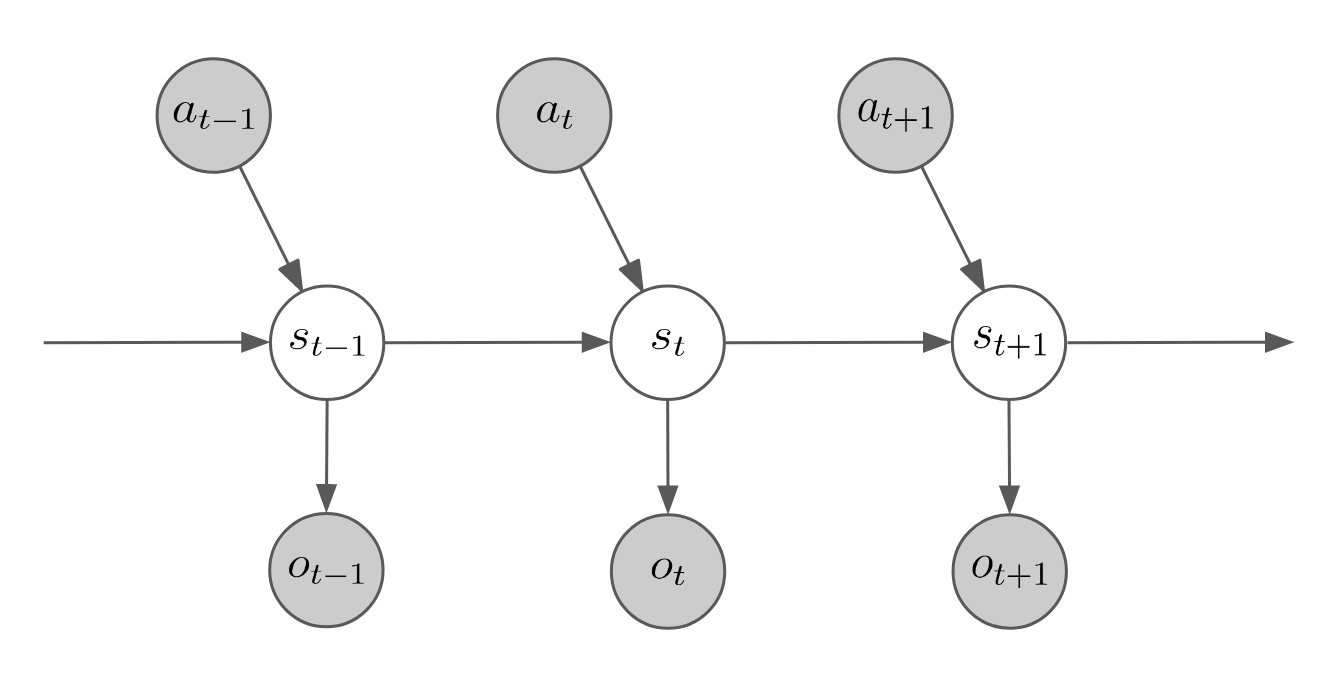
\includegraphics[width=0.9\linewidth]{./figures/dssm.png}
      \caption[DSSMのグラフィカルモデル]{DSSMのグラフィカルモデル.実線は生成分布,点線は推論分布を表す.}
      \label{fig:ssm}
    \end{center}
  \end{figure}

\section{深層状態空間モデルの問題点}
深層状態空間モデルを用いてより複雑な環境の映像予測を考える場合,潜在的な情報が多くなるはずであるためより大きな状態表現を扱えるようモデルを大きくする必要がある.素朴には状態変数の次元を大きくすることがよいと考えられるが,予備実験の中で深層状態空間モデルは状態変数の次元を大きくすると学習が困難になる,または学習が安定しにくくなることがわかった.まずこのことを示した上で,この理由を考察する.

\begin{figure}[bp]
  \begin{center}
    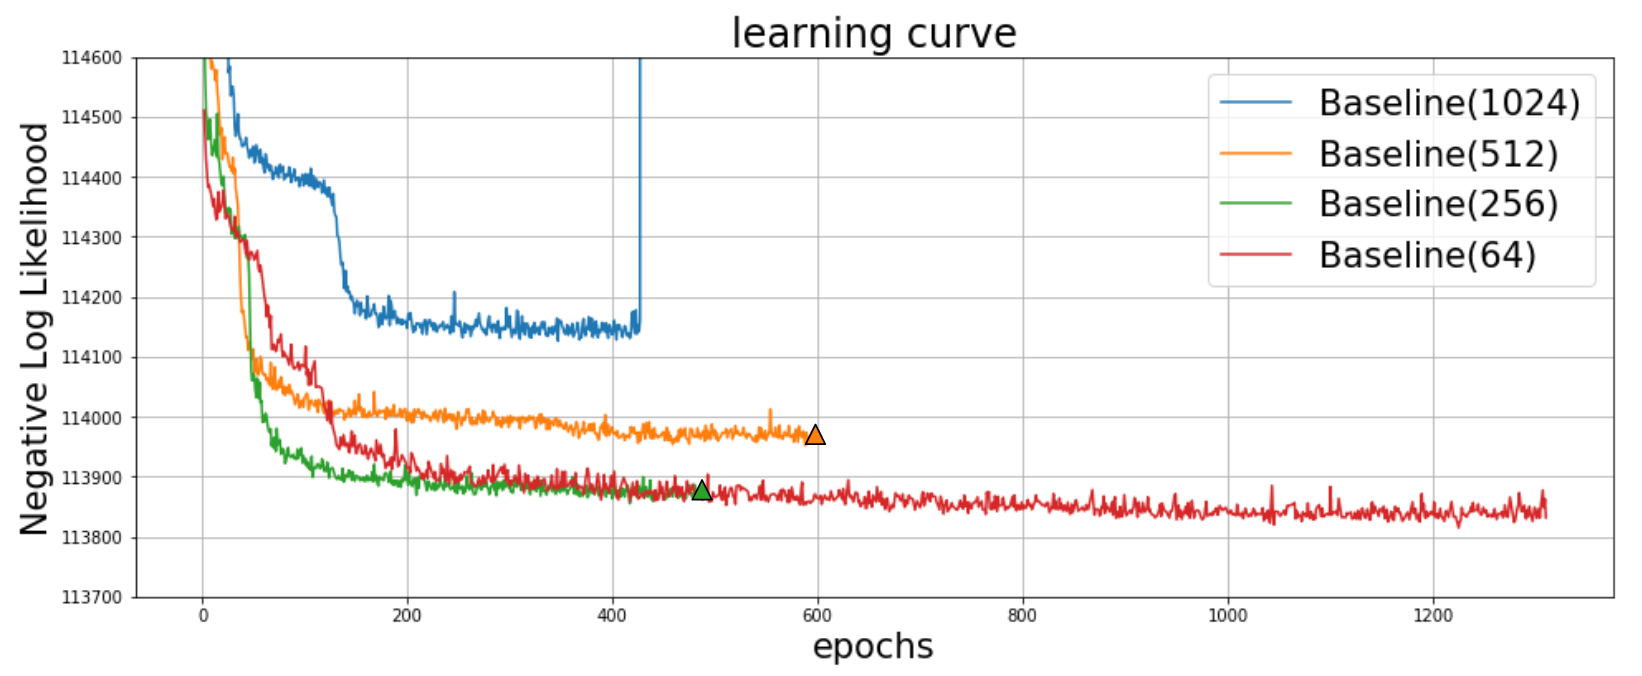
\includegraphics[width=\linewidth]{./figures/dssm_curve_yoko.png}
    \caption[状態変数の次元を変えた時のDSSMの学習曲線]{状態変数の次元を変えた時のDSSMの学習曲線.横軸がepoch数で縦軸が目的関数の値である.グラフ中に三角で示されるのは目的関数の値にNanが出力されてしまったことを示す.}
    \label{fig:dssm_curve}
  \end{center}
\end{figure}

\subsection{学習が失敗した例}
図 \ref{fig:dssm_curve}は,本論文の4章以降でベースラインとして用いる通常のDSSMモデルを状態変数の次元を何通りかに変えてモデルを構築し,学習時の訓練用データでの目的関数の値の増減をプロットしたものである.状態変数を比較的低次元の64次元に設定すると順調に学習が進み,図 \ref{fig:dssm_base}の左図に示すように少しずつ近い映像が出力されるようになる.しかし状態変数の次元を512次元に設定すると明らかに精度が悪化し,1024次元にするとさらに悪化している.図 \ref{fig:dssm_base}の右図は1024次元での実験で目的関数の値が発散した後の生成映像の様子で,他の次元で学習が失敗した場合も同じような映像が生成される.256次元や512次元での実験で途中から目的関数の値にNanが出力されてしまうのは,5章の「実験の安定化」で述べるように,カルバックライブラー距離を小さくすることに失敗しゼロ除算が発生したためである.1024次元で値が発散している理由は定かでないが,256次元,512次元と同様の理由であると考えられる.

\begin{figure}[tp]
  \begin{minipage}{0.48\hsize}
    \begin{center}
      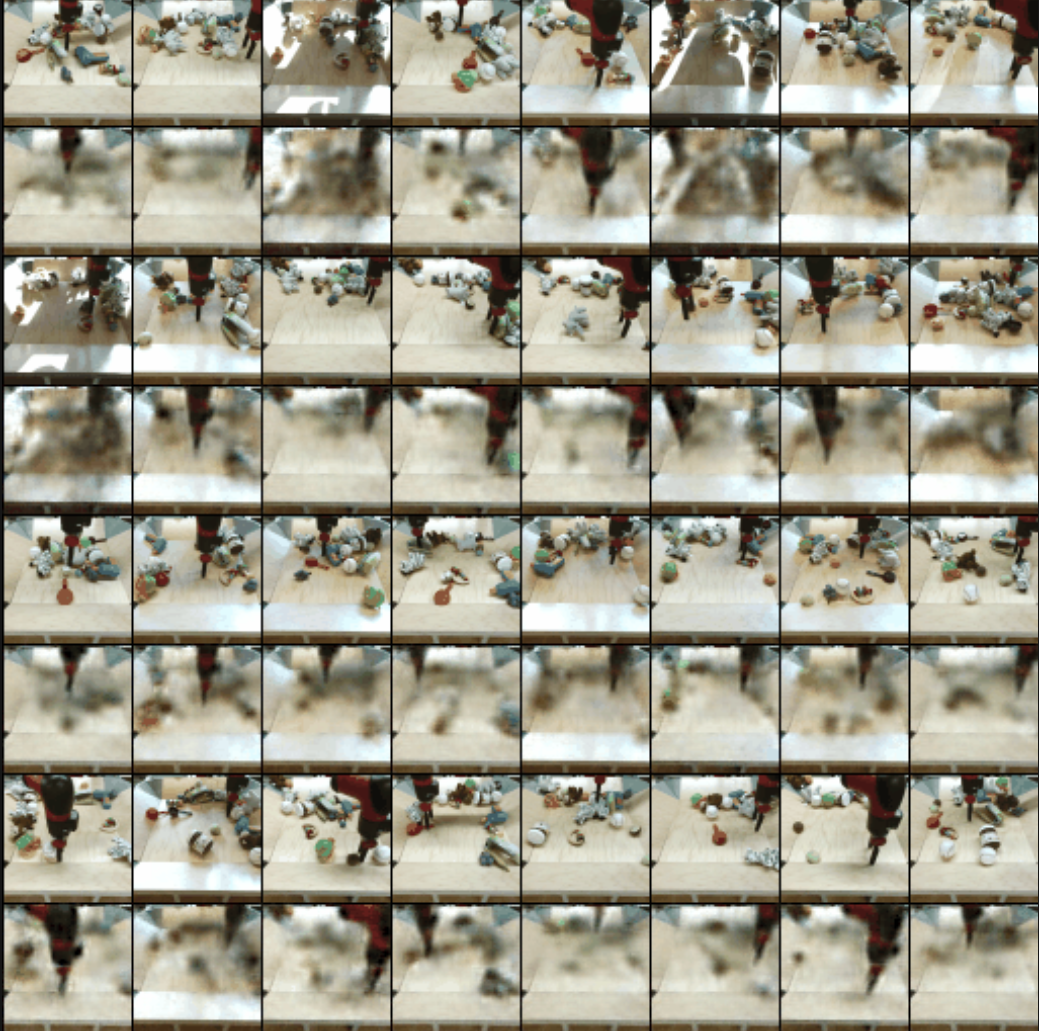
\includegraphics[width=\linewidth]{./figures/dssm_64.png}
      \caption{(a) 学習が進んでいる例}
    \end{center}
  \end{minipage}
  \begin{minipage}{0.48\hsize}
    \begin{center}
      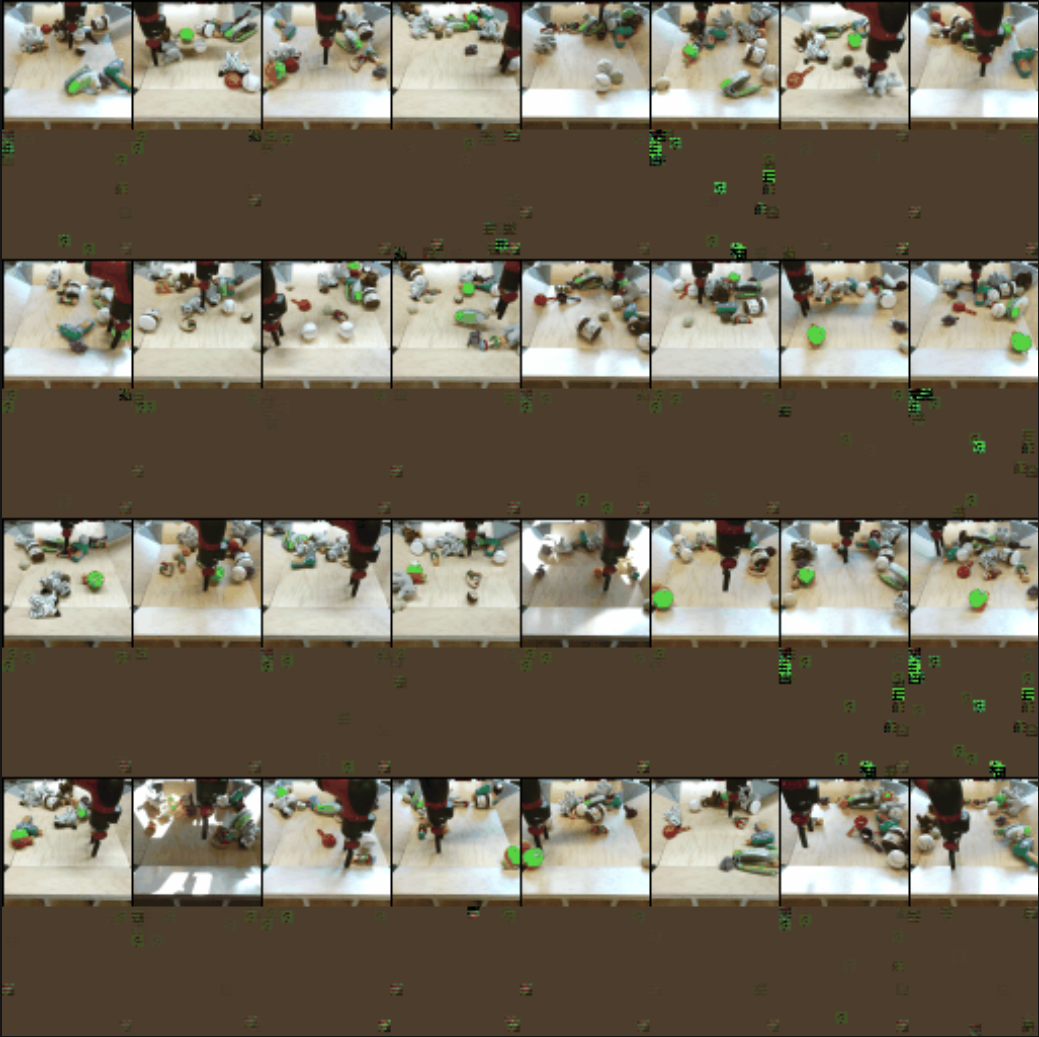
\includegraphics[width=\linewidth]{./figures/dssm_1024.png}
      \caption{(b) 学習が失敗した例}
    \end{center}
  \end{minipage}
  \label{fig:dssm_base}
  \caption[DSSMの学習中にサンプルされた映像の例]{DSSMの学習中にサンプルされた映像の例.上から奇数段目が正解映像で,上から偶数段目が一段上の映像の行動条件付き予測結果である.10フレームの映像予測を行っているが,図ではある一時刻の観測のみが示されている}
\end{figure}

ELBOがNanをとったり発散したりすることは数値計算の丸め誤差などの理由も関わるので一旦考えないとしても,明らかに状態変数の次元を大きくすることで精度が下がっていることが図 \ref{fig:dssm_curve}からわかる.

\subsection{学習が難しくなる理由の考察}
VAEの学習では前節で述べたような問題は起こらないことを踏まえると,DSSMで学習が難しいのは状態変数の遷移の部分であると考えられる.さらに,状態変数に高次元を仮定したとき,状態変数の遷移の部分では状態変数の生成モデル・推論モデルともに高次元ベクトルから高次元ベクトルへの写像を学習する必要が生じてまずこの部分で学習に時間がかかりやすくなっており,さらに推論モデルが十分に学習されないまま状態変数の事前分布と事後分布のカルバックライブラー距離の最小化が図られてしまうので,学習が安定しにくなっていると考えられる.

このことから,単に状態変数を高次元にすることはDSSMの性質上適切ではなく,DSSMをより複雑な環境を扱う問題にスケールさせるためには他の方法を考える必要がある.以上の予備実験を受け,次章ではシンプルなDSSMの拡張方法を提案する.

\section{状態表現の階層性を考慮することによる深層状態空間モデルの拡張}
\label{chap:proposal}

第三章の問題を受け,第四章ではシンプルな帰納バイアスを導入することによってDSSMを拡張する方法を提案する.はじめに本研究で扱う問題設定について改めて整理し,続けて提案手法とその既存の類似手法について述べる.

\subsection{問題設定}

本研究では行動条件付き映像予測の問題を解く.具体的には,ある行動主体が実行した行動系列$a_{1:10}$と初期観測$o_0$が与えられたときに$o_{1:10}$を生成し,その生成される映像の尤度を高めることを目指す.ただし訓練時には行動系列と観測系列の組$\{\vec{a}, \vec{o}\}$の訓練用のデータセットを用いることができ,評価時には,訓練データには含まれないが訓練データと同じ条件で収集された評価用のデータセットを用いる.
本研究の目的は,この条件付き映像予測問題においてベースラインにDSSMを設定し,DSSMをより複雑な環境での映像予測問題にもスケールできるように拡張することである.

\subsection{提案手法}
三章で述べたようにベースラインのDSSMでは潜在変数の次元を大きくすると学習がうまくいかなかった.しかし予備実験で得た,低次元の潜在変数を用いたときには部分的に学習が進んだという事実をヒントにし,状態変数の次元を大きくしていく方向性はそのままで状態表現の階層性を考えることにより,より複雑な問題設定においても学習可能なDSSMの拡張方法を提案する.

\begin{figure}[tp]
  \begin{center}
    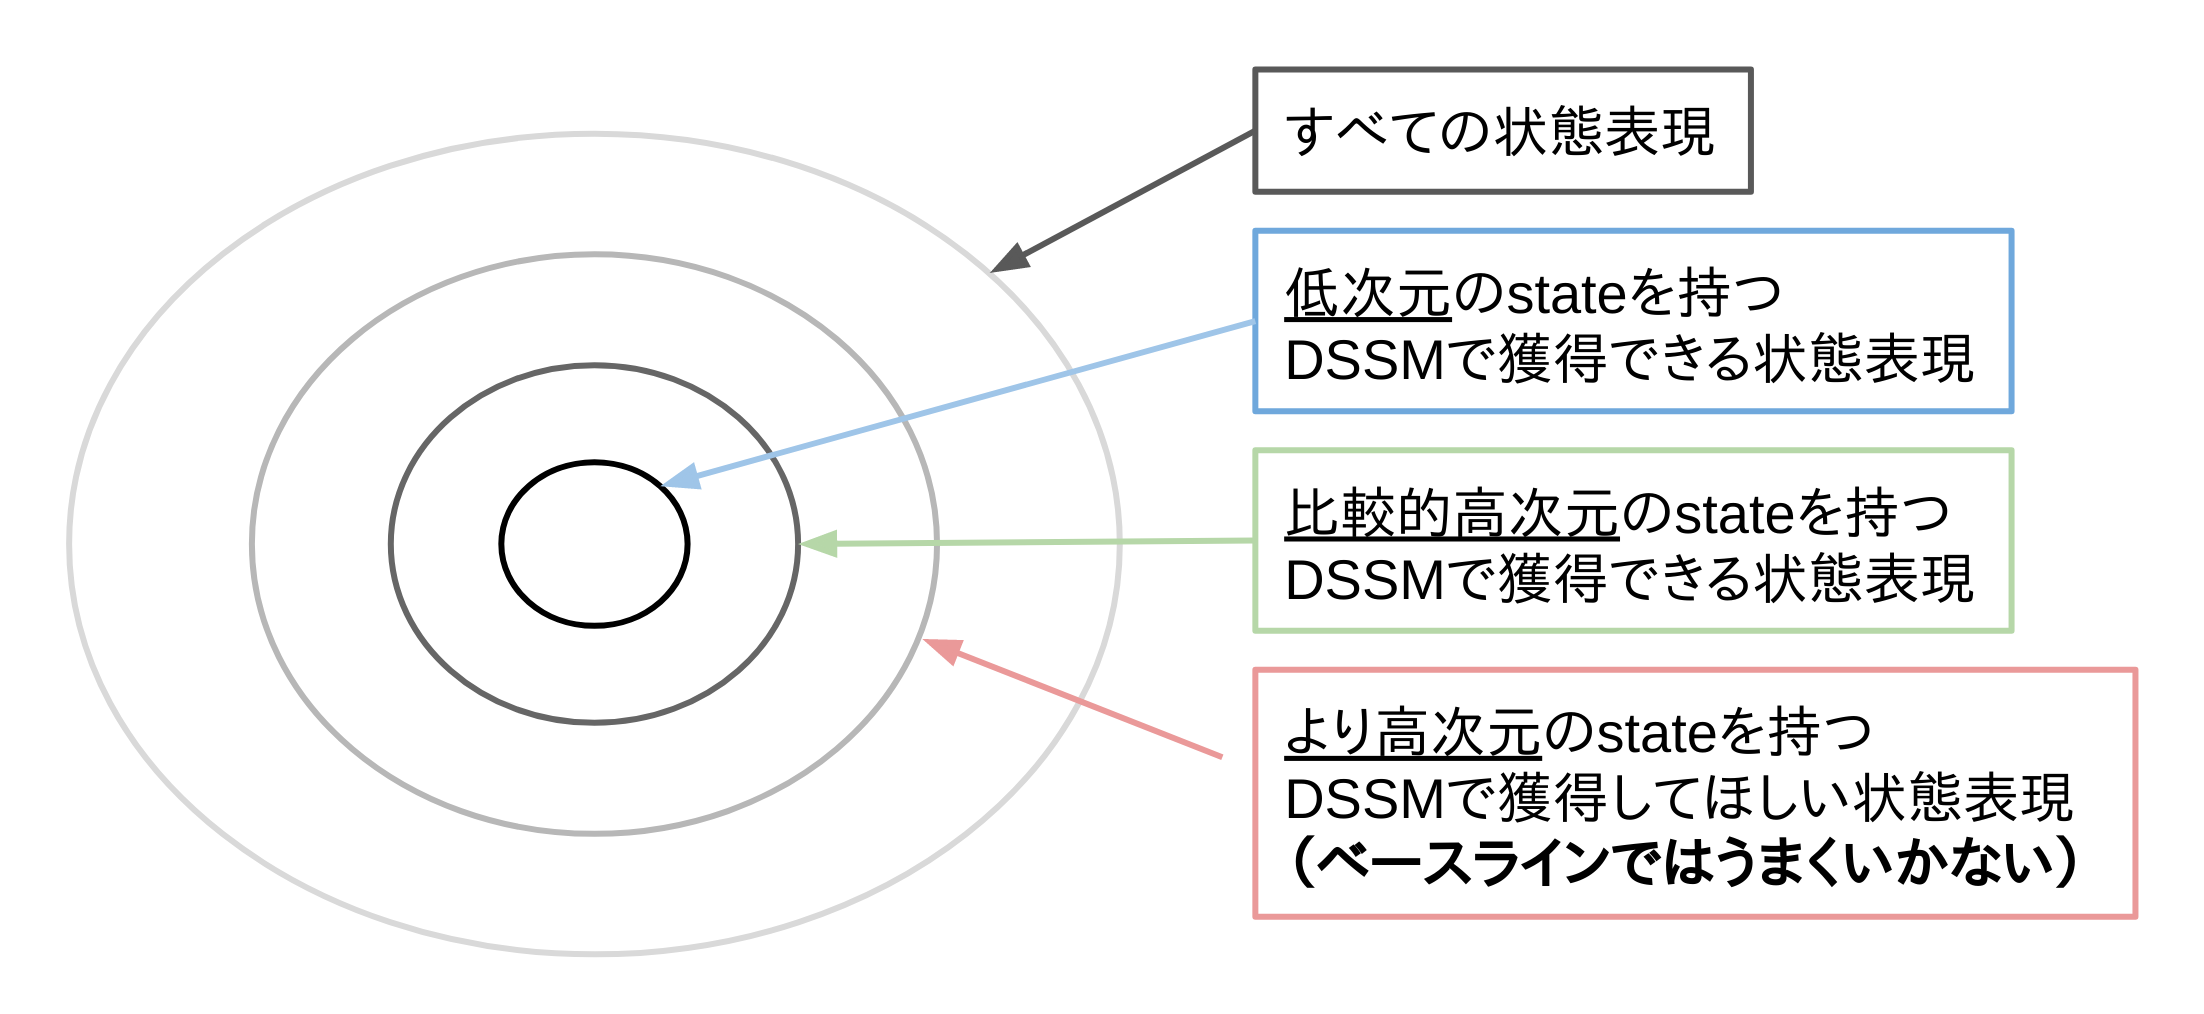
\includegraphics[width=\linewidth]{./figures/hierarchical.png}
    \caption{獲得される状態表現の包含関係}
    \label{fig:hierarchical}
  \end{center}
\end{figure}

\subsection{状態表現の階層性}
はじめに,ベースラインのDSSMにおいて潜在変数の次元を変えた時に獲得される情報について考察する.低次元の状態変数で獲得できる情報は高次元の状態変数を用いた場合にも当然獲得できると考えた場合,図(\ref{fig:hierarchical})のように高次元の状態変数が持つ情報は低次元の状態変数が持つ情報をほぼ内包していると考えることができる.
ここで状態変数の次元をより大きくしたときに精度がむしろ悪化することが問題であったが,これは三章で述べたとおり,状態変数の次元が大きくなったときに高次元ベクトルから高次元ベクトルへの写像を学習する必要が生じあるべき写像先がなかなか定まらないことが原因であると考えられ,何らかの方法で遷移モデルの学習を補助することで図のようにより多くの情報を獲得できる可能性がある.

\subsection{階層的な状態表現の遷移}
ベースラインの状態表現の遷移は図(\ref{fig:transition_base})が示すように状態変数が持つすべての情報を一度に変換することを考えているが,直感的に一括で変換することは学習が難しいと思われる.状態表現を一括で変換する代わりに,前節のような階層性の概念を導入することで図(\ref{fig:transition_proposal})のように簡単に遷移が学習できる部分から順に遷移させていくような方法を考えることができる.

このような階層的な状態表現の遷移を考えると,はじめから高次元の状態表現の遷移を考えずに学習の習熟度に合わせて徐々に高次元の状態ベクトルの遷移を学習することができ,学習がスムースに進みやすくなると考えられる.

% \begin{figure}[tbp]
%   \begin{center}
%     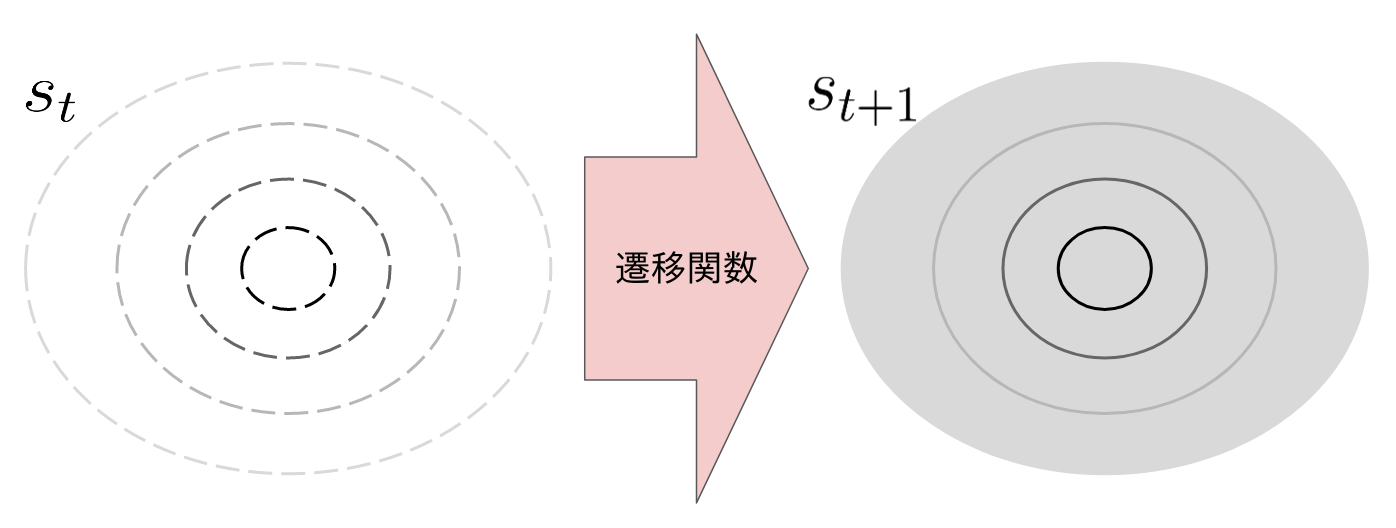
\includegraphics[width=0.5\linewidth]{./figures/transition_base.png}
%     \caption{ベースラインの状態遷移の模式図}
%     \label{fig:transition_base}
%   \end{center}
% \end{figure}

% \begin{figure}[tbp]
%   \begin{center}
%     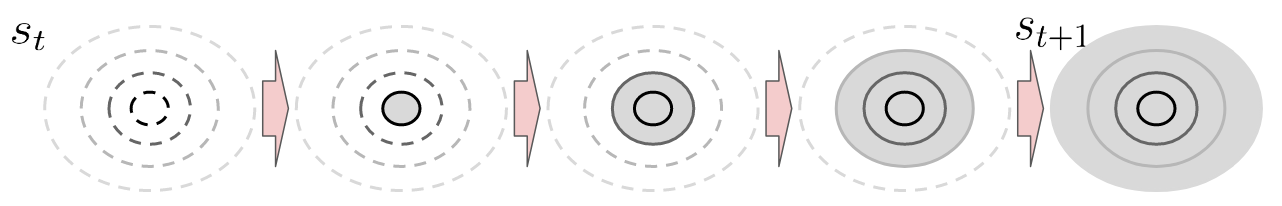
\includegraphics[width=0.8\linewidth]{./figures/transition_proposal.png}
%     \caption{提案手法の状態遷移の模式図}
%     \label{fig:transition_proposal}
%   \end{center}
% \end{figure}

% \caption[hoge]{fuga}
\begin{figure}[tbp]
  \begin{center}
    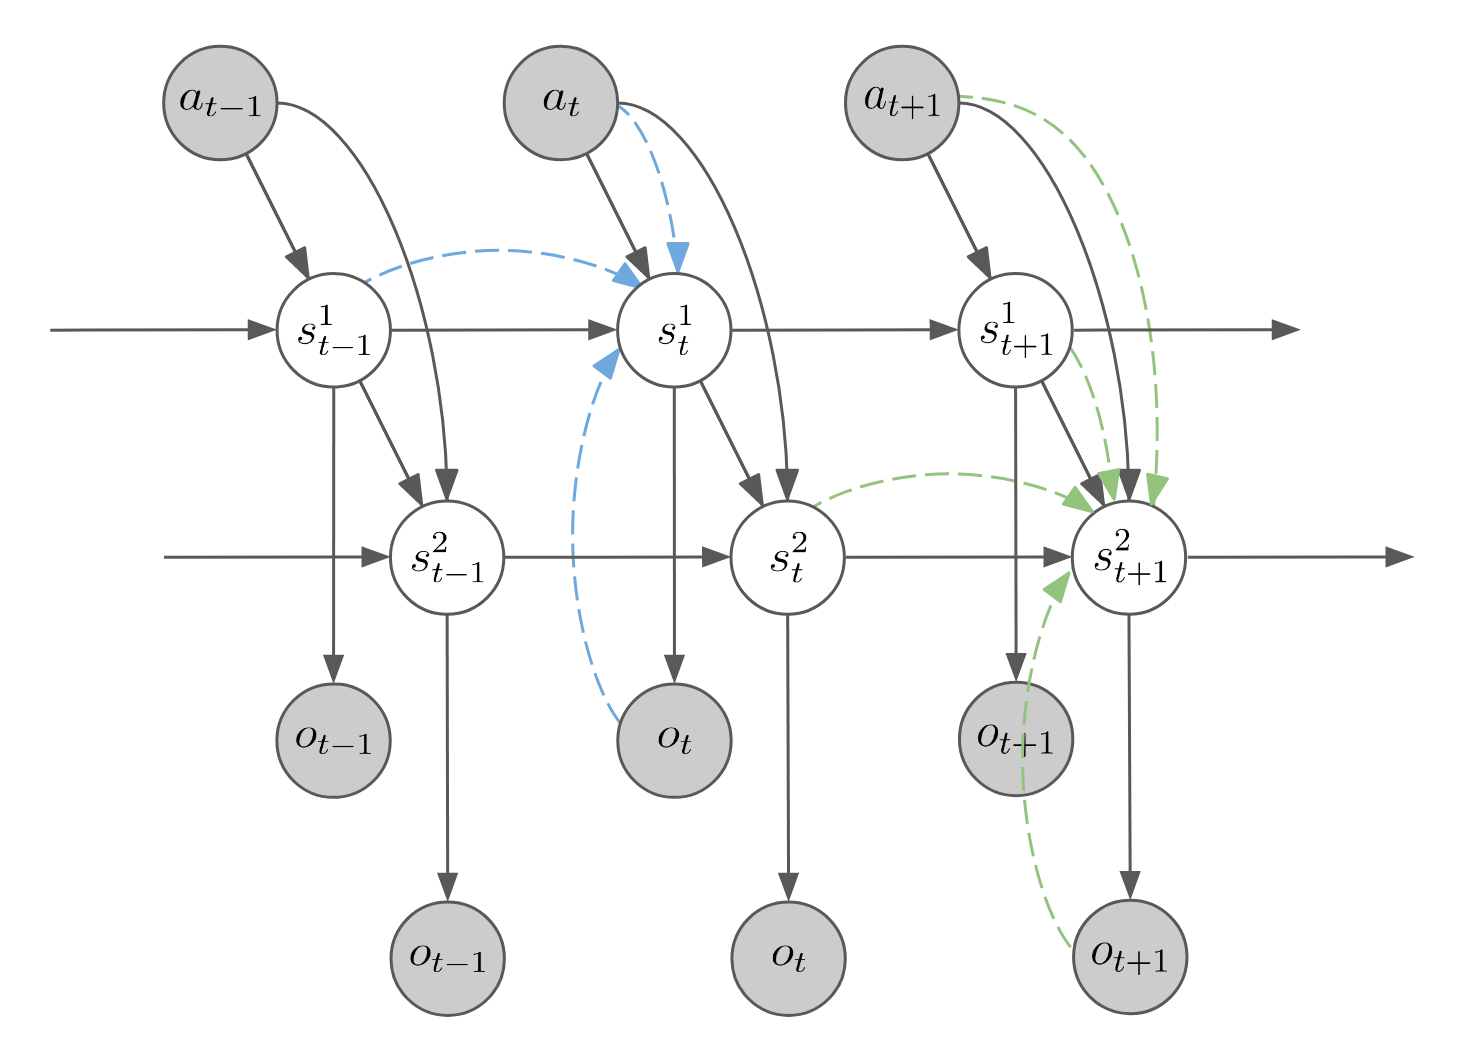
\includegraphics[width=\linewidth]{./figures/proposal_train.png}
    \caption[提案手法(二階層)のグラフィカルモデル]{提案手法のグラフィカルモデル.実線が生成分布,点線が推論分布を示す.$s^1$, $s^2$の推論分布は簡単のため時刻t, t-1でのみ記載している.また2つずつ記載されている$o_t$は同じデータを示すが.異なるsから独立に生成されることを明示している.}
    \label{fig:proposal}
  \end{center}
\end{figure}

\subsection{確率モデル・最適化}

ここまでで状態変数の階層性とその遷移を考えたが,この階層性の仮定はDSSMの性能の向上に十分寄与しうると考え,状態変数の階層性を帰納バイアスとしてDSSMに組み込み以下のようなモデルとその最適化アルゴリズムを提案する.

\vspace{\baselineskip}
提案手法のグラフィカルモデルを図(\ref{fig:proposal})に示す.提案手法は,DSSMの状態変数をN層に階層化したモデルである.図(\ref{fig:proposal})は2階層の提案モデルを表している.図(\ref{fig:proposal})の上側の状態変数から一階層の状態変数・二階層の状態変数と呼ぶことにすると一階層の状態変数が低次元ベクトル,二階層の状態変数が高次元ベクトルになっており,高次元の状態変数の生成・推論時に低次元の状態変数を用いるようなモデルになっている.高次元の状態変数の遷移時に低階層の状態変数を用いて写像先に関する情報を補助的に与えることで,学習を安定化させる効果が期待される.またモデルの評価時には,最高層の観測の生成モデル $p(o_t|s^N_t)$ を用いる.

\begin{algorithm}[tbp]               
  \caption{N階層DSSMの学習アルゴリズム}
  \label{alg1}
  \begin{algorithmic}
    \REQUIRE 階層数 $N$ 
    \FOR{i = 1 to $N$}
      \WHILE{$i$階層のネットワークの学習が収束していない}
        \STATE $1 \sim i-1$階層のネットワークのパラメータを固定し, 
        \STATE $i$階層のネットワークを以下の目的関数で学習する
        \STATE $L(a_{1:T}, o_{1:T}) = $
        % \STATE $ \hspace{2em}\sum_{t=1}^T ( \mathbb{E}_{s^i_t} [\log p(o_t|s^i_t)] - \mathbb{E}_{s^i_{t-1}} [\mathrm{D_{KL}}(q(s^i_t|s^i_{t-1}, a_t, o_t) \| p(s^i_t|s^i_{t-1}, a_t, o_t, s^{i-1}_t)]) $
      \ENDWHILE
    \ENDFOR
  \end{algorithmic}
\end{algorithm}

\vspace{\baselineskip}
次に提案手法の学習アルゴリズムをアルゴリズム\ref{alg1}に示す.この学習アルゴリズムは前節「階層的な状態表現の遷移」で述べた,習熟度に合わせて徐々に高次元の状態ベクトルの遷移を学習するという考え方に基づいており,これにより安定した学習が見込める.今回簡単のために高階層の潜在表現の学習時にはそれより低階層の状態表現の学習を止めているが,他の方法も考えられ,これついては考察「低次元状態ベクトルの階層の再学習」で述べる.

\section{実験}
\label{chap:experiment}
第4章で述べた提案手法の有効性を検証するために,BAIR Push Dataset\cite{ebert2017selfsupervised}という行動条件付き映像予測用のデータセットを用いて評価実験を行った.本章では実験の内容について説明した後に実験結果について述べる.

\subsection{実験内容}
第4章で述べた提案手法とベースラインの比較を行う.ベースラインは第二章で述べたシンプルなDSSMとし,状態ベクトルの次元を64, 256, 512, 1024の4通りに変えて実験を行う.提案手法は64次元と512次元の二階層の状態ベクトルを持つモデルと,64次元と512次元と1024次元の三階層の状態ベクトルを持つモデルとした.ベースラインと提案手法の実装の差は必要最小限にとどめ,どちらも学習時には10フレーム先までの予測を行った.またパラメータの最適化にはそれぞれ確率的勾配降下法アルゴリズム Adam\cite{kingma2014adam} を用いた.評価の際には,定量評価として予測誤差(負の対数尤度)を測り,合わせて定性評価も行う.

\subsubsection{データセット}

今回用いるBAIR Push Dataset\cite{ebert2017selfsupervised}は行動条件付き映像予測と行動条件をつけない映像予測のどちらの研究でも用いられるデータセットであり,カリフォルニア大学バークレー校によって制作・公開されている.
こちらのデータセットは,様々な物体がおかれた机の上をロボットアームがランダムに掻き乱すようにして様々なデータが記録されており,今回はその中から行動系列$\vec{a}$と固定視点から観測された画像系列$\vec{o}$を用いる.今回用いる行動系列$\vec{a}$は,具体的にはロボットのエンドエフェクタの位置姿勢の命令値になっている.観測画像は64x64サイズのRGB画像で,これらのデータは10hzで撮られている.また訓練時と評価時に使われる物体は揃えられている.

\subsubsection{ベースラインの実装}
深層学習フレームワークPytorch\cite{pytorch}と,深層生成モデルライブラリPixyz\cite{pixyz}を主に用いた.学習用データの読み込みとその最適化には深層学習フレームワークTensorFlow\cite{tensorflow}を用いた.また実装では,DSSMを用いた強化学習手法であるPlaNetの公開実装\cite{planet}を参考にした.
まずベースラインの実装を説明した後,提案手法の実装について述べる.

\subsubsection{モデルアーキテクチャ}
ベースラインは4つの部分モデルから構成される.
% \begin{itemize}
%     \item デコーダー $p(s_t|x_t)$
%     \item エンコーダー $q(x_t|h_t)$
%     \item 遷移モデル(事前分布) $p(s_t|s_t-1, a_t)$
%     \item 遷移モデル(事後分布) $q(s_t|s_t-1, a_t, h_t)$
% \end{itemize}

遷移モデル(事前分布)とデコーダーが生成モデルに相当し,提案手法のグラフィカルモデルの実践部分を表しす.遷移モデル(事後分布)とエンコーダーが推論モデルに相当し,提案手法のグラフィカルモデルの点線部分を表している.

\subsubsection{学習の安定化}
潜在変数の次元を大きくした際,学習の初期段階でカルバックライブラー距離の計算値が発散することがよく起こる.これは遷移モデルが次の時刻の状態ベクトルの分布の標準偏差として0に非常に近い値を出力してしまった結果(丸め誤差が発生して)カルバックライブラー距離の計算時にゼロ除算が発生してしまうためである.この問題は遷移モデルが出力する標準偏差に下限を設けることで解決することができる.今回の実験では潜在変数の次元を1024次元にした際にこのカルバックライブラー距離が学習開始後直ちに発散する問題が発生したので,標準偏差の下限値を$10^{-7}$とすることで学習をある程度継続することができた.ただし標準偏差に下限を設けることは経験的に学習を難しくすることがわかっていたので,他の条件での実験の際には適用しなかった.

\subsection{提案手法の実装}
提案手法はベースラインの節で説明した部分モデルをほぼそのまま用いる.二階層目以上の第i層では,各遷移モデルの入力として一時刻前の状態変数$s^i_{t-1}$と行動$a_t$だけでなく,一つ低次元の層の同じ時刻の状態ベクトル$s^{i-1}_t$も入力とする.また,提案手法では,パラメータを固定している層の状態ベクトルのサンプリングには,モデルの評価時の設定に合わせて常に事前分布を用いている.これは,パラメータを固定している層はそれ以上学習されないために,事前分布より良い表現が下の階層に渡されることはなく,むしろ事前分布で足りない表現を積極的に下の階層の学習で獲得できるようにするためである.
その他はベースラインの実装と変えていない.


\section{実験結果}

簡単のため,ここから状態変数の次元を64にしたベースラインモデルを「ベースライン(64)」,状態変数の次元を64と512にした提案手法モデルを「提案手法(64 + 512)」などと呼ぶ.

\subsection{定量評価(尤度)}

\begin{figure}[tp]
    \begin{center}
        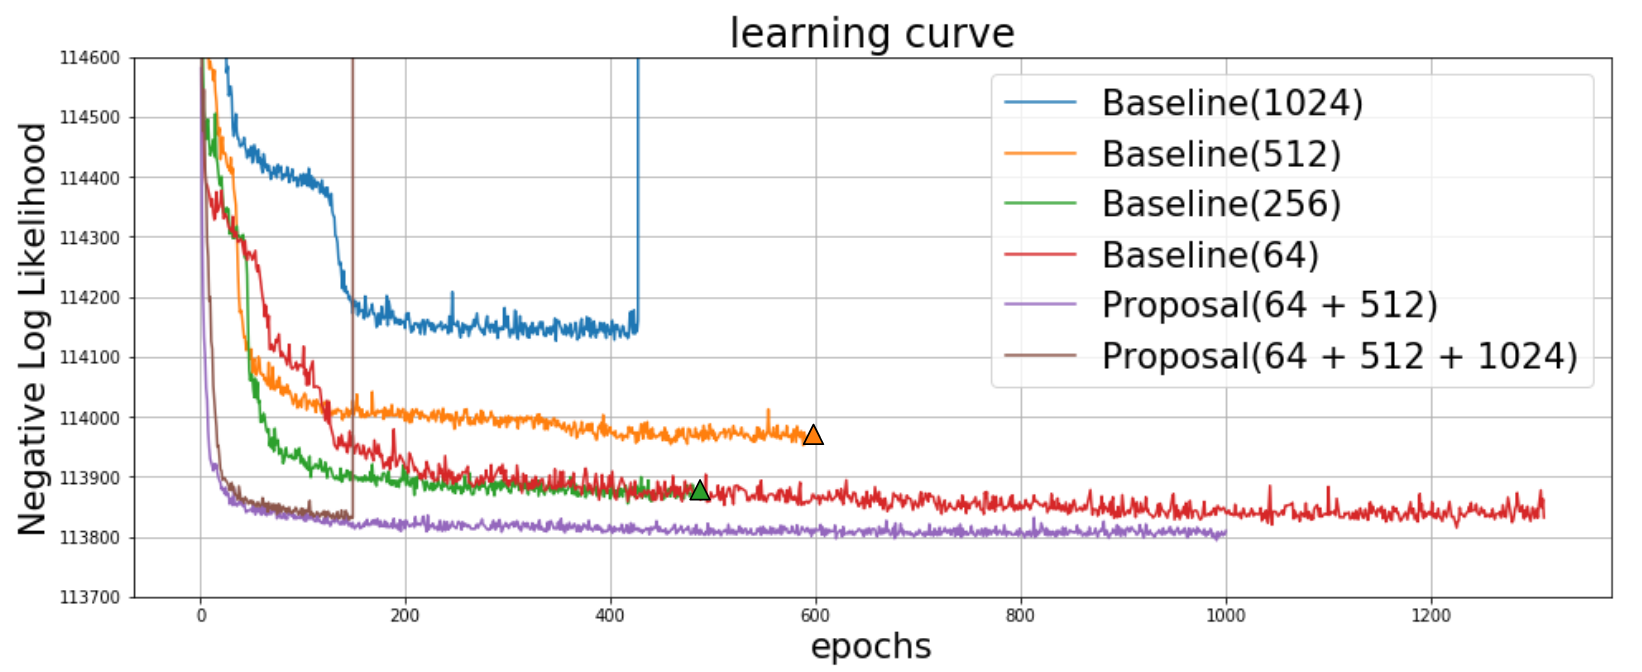
\includegraphics[width=\linewidth]{./figures/curve_yoko.png}
        \caption[提案手法の学習曲線]{ベースラインと提案手法の学習曲線}
        \label{fig:curve}
    \end{center}
    \end{figure}

\begin{table}[tbp]
    \begin{center}
    \caption{手法ごとの定量評価指標(尤度)}
    \begin{tabular}{|c||c|} \hline
      手法 & 負の対数尤度 \\ \hline \hline
      ベースライン(64) & $1.1384 \times 10^5 $ \\ \hline
      ベースライン(256) & $1.1387 \times 10^5 $ \\ \hline
      ベースライン(512) & $1.1397 \times 10^5 $ \\ \hline
      ベースライン(1024) & $1.1416 \times 10^5 $ \\ \hline
      提案手法(64 + 512) & $\bm{1.1381 \times 10^5 }$ \\ \hline
      提案手法(64 + 512 + 1024) & $1.1383 \times 10^5$ \\ \hline
    \end{tabular}
    \label{table:evaluation}
    \end{center}
  \end{table}
  

図(\ref{fig:curve})は,ベースラインと提案手法の学習時の評価用データでの負の対数尤度の値の推移をプロットしたもの(学習曲線)である.ただし提案手法(64 + 512)は一階層部分に1000 epoch 学習したベースライン(64)を用いており,学習曲線としてプロットされているのは二階層部分の学習時の負の対数尤度である.同様に提案手法(64 + 512 + 1024)は一階層部分に1000 epoch 学習したベースライン(64)を,二階層部分に1000 epoch 学習した提案手法(64 + 512)を用いており,学習曲線としてプロットされているのは三階層部分の学習時の負の対数尤度である.また表(\ref{table:evaluation})に最終的な負の対数尤度を示す.

まず図(\ref{fig:curve})について,ベースライン(512)と提案手法(64 + 512)との比較から,二階層にすることで潜在変数の次元を512次元と大きくした際にもうまく学習が進むようになったことがわかる.これは,高次元の状態変数の学習時に学習済みの低次元の状態変数の情報を用いることで狙い通り学習が安定したためだと考えられる.次にベースライン(64)と提案手法(64 + 512)の比較から,高次元の潜在変数で学習させたことによってより高い尤度の映像を生成できるようになったことがわかる.これは潜在変数を高次元にした方が多くの情報を保持しやすく,適切に学習が進みさえすれば予測性能が向上しやすくなるためだと考えられる.最後に三階層の提案手法(64 + 512 + 1024)について見ると,ベースライン(1024)と比較し明らかに学習が進んだものの,ベースライン(64 + 512)と比較して精度の改善は見られず,潜在変数の次元を大きくすることだけでは精度の向上には限界があるということが伺える.

\subsection{定性評価}
図(\ref{fig:compare_ad})は評価用データで10フレームの行動条件付き映像予測により生成された映像のサンプルで,正解映像とベースライン(64)による予測映像,提案手法(64 + 512)による予測映像を比較している.どちらのモデルもロボットアームの位置はほぼ正しく予測ができているが,環境中の物体の見た目には差が見られた.図(\ref{fig:pred_a}), 図(\ref{fig:pred_b})を見ると,ベースラインでは環境中の物体の輪郭がぼやけて灰色がかっているのに対し,提案手法では特に物体が密集していない場合に比較的物体一つ一つの生成が鮮明になっていることが見て取れる.これは潜在変数の次元を大きくし保持できる情報を増やすことに成功したためだと言える.しかしフレームごとの見た目には改善が見られたものの,物理的な操作についての予測はあまり改善が見られなかった.図(\ref{fig:pred_c})では,正解映像ではロボットアームの移動によって中央の緑の物体の姿勢を変えているが,そもそもベースラインではその物体を生成できておらず,提案手法でも僅かに黒っぽい点として表されている程度で姿勢の変化を読み取ることはできない.図(\ref{fig:pred_d})は,正解映像では滑らせるようにして2つの物体を近づけており,提案手法のでは2つの物体の輪郭が見られるが,机の色やロボットアームの色と途中から同化してその動きを追うことは困難である.このように物理的な操作の予測を改善するにはまず一フレーム一フレームの質を上げる必要があると考えられ,今回は物理的な操作の予測の改善はあまり見られなかった.最後に図(\ref{fig:pred_long})は,各モデルで学習時よりも長い30フレームの映像予測をした際の生成映像である.ベースライン・提案手法ともにロボットアームの動きはほぼ正解映像と一致しているが,ベースラインでは右端に映る物体が映像を予測するにつれて青色から緑色に変わってしまっているのに対し,提案手法は背景や周りの物体について一貫性が保たれていた.これは,潜在変数の次元が小さいまま性能をあげようとすると潜在表現に含まれる情報が密になりすぎて遷移時に遷移とは関係のない情報も変化させてしまいやすいという問題がある可能性があり,一方提案手法は高次元の潜在変数を使うためにそのような問題は生じなかったと考えられる.

% また図(\ref{fig:pred_a})では,水色の物体の予測位置が提案手法が生成した映像と正解映像とで少しずつずれているが,このことから画像を一画素ずつ潜在表現で記憶しているのではなく,物体の見た目と位置を別々に保存するように学習がすすんでいたことが伺える.

% 高次元で学習できるようになった.これは深層状態空間モデルの大きな問題点を克服できたと言える.

\begin{figure}[tp]
    \centering
    \subfloat[]{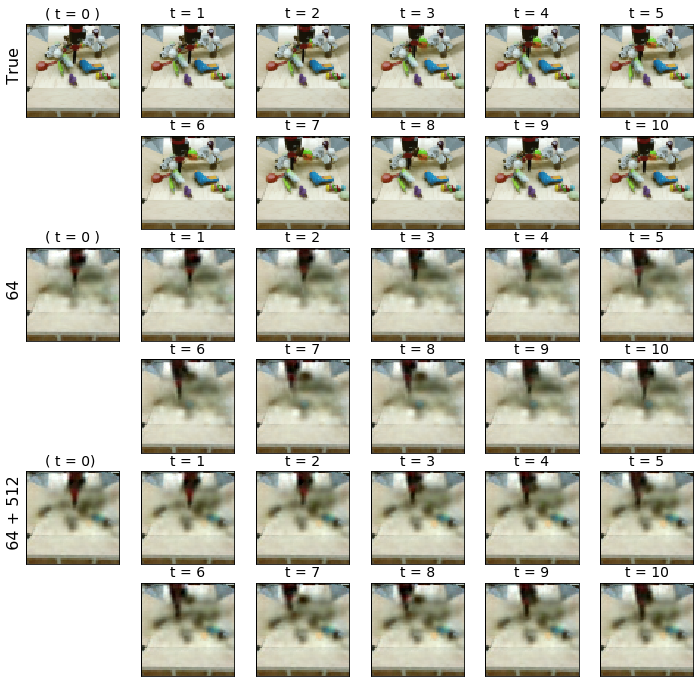
\includegraphics[clip, width=0.95\linewidth]{./figures/pred_a.png}
    \label{fig:pred_a}}
    \\
    \subfloat[]{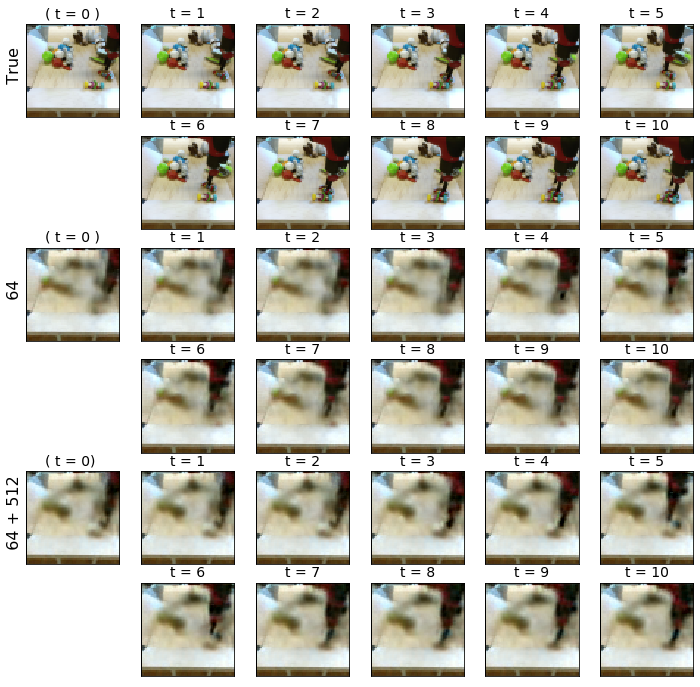
\includegraphics[clip, width=0.95\linewidth]{./figures/pred_d.png}
    \label{fig:pred_d}}
    \caption[映像予測結果1]{映像予測結果1.「True」が正解映像,「64」がベースライン(64)での予測結果,「64 + 512」が提案手法(64 + 512)での予測結果を示す.また$t = 0$は初期状態の推論時に与えられるフレーム.}
    \label{fig:compare_ad}
\end{figure}

\section{考察}
課題メイン

\section{結論}

本論文では,実機ロボットへの応用を見据えて深層状態空間モデルを用いた映像予測について取り上げた.まず深層強化学習などで用いられているシンプルな深層状態空間モデルでは複雑な環境を扱う問題設定に上手くスケールしない問題を示し,その上で深層状態空間モデルの状態表現の階層性を明示的にモデル化した提案手法によってより高次元の状態表現を扱えるようにし,さらに映像予測の性能が向上することを示した.
実験では,定性的な大きな優位性は示せなかったものの,高次元の状態変数を用いた学習を可能にしたことは深層状態空間モデルの大きな問題を克服したと言える.これにより,これまで映像予測の分野では実機ロボットへの応用上の制約が多いにも関わらず自己回帰的なモデルの研究が主流であったが,状態空間モデルベースの手法が見直されるきっかけになるかもしれない.

第六章では展望として深層状態空間モデルの研究の方向性を複数上げたが,これらの研究をすすめることによってより高性能な予測が可能になり,また実機への応用の可能性も高められると考える.さらに社会応用の例として,映像予測の実機応用に加え,新たな物理シミュレーションの近似アプローチと新たなロボット学習のあり方の可能性について述べた.この二つの応用例は現段階では可能性の話に過ぎず実現可能かは定かでないがどちらも実現すれば社会的な価値は大きいと考えられるので,今後も慎重に研究を継続していきたい.

\bibliography{references}
\bibliographystyle{unsrt}
%%%%%%%%%%%%%%%%%%%%%%%%%%%%%%%%%%%%%%%%%%%%%%%%%%
\end{document}